% Options for packages loaded elsewhere
\PassOptionsToPackage{unicode}{hyperref}
\PassOptionsToPackage{hyphens}{url}
%
\documentclass[
]{article}
\usepackage{amsmath,amssymb}
\usepackage{lmodern}
\usepackage{iftex}
\ifPDFTeX
  \usepackage[T1]{fontenc}
  \usepackage[utf8]{inputenc}
  \usepackage{textcomp} % provide euro and other symbols
\else % if luatex or xetex
  \usepackage{unicode-math}
  \defaultfontfeatures{Scale=MatchLowercase}
  \defaultfontfeatures[\rmfamily]{Ligatures=TeX,Scale=1}
\fi
% Use upquote if available, for straight quotes in verbatim environments
\IfFileExists{upquote.sty}{\usepackage{upquote}}{}
\IfFileExists{microtype.sty}{% use microtype if available
  \usepackage[]{microtype}
  \UseMicrotypeSet[protrusion]{basicmath} % disable protrusion for tt fonts
}{}
\makeatletter
\@ifundefined{KOMAClassName}{% if non-KOMA class
  \IfFileExists{parskip.sty}{%
    \usepackage{parskip}
  }{% else
    \setlength{\parindent}{0pt}
    \setlength{\parskip}{6pt plus 2pt minus 1pt}}
}{% if KOMA class
  \KOMAoptions{parskip=half}}
\makeatother
\usepackage{xcolor}
\usepackage[margin=1in]{geometry}
\usepackage{color}
\usepackage{fancyvrb}
\newcommand{\VerbBar}{|}
\newcommand{\VERB}{\Verb[commandchars=\\\{\}]}
\DefineVerbatimEnvironment{Highlighting}{Verbatim}{commandchars=\\\{\}}
% Add ',fontsize=\small' for more characters per line
\usepackage{framed}
\definecolor{shadecolor}{RGB}{248,248,248}
\newenvironment{Shaded}{\begin{snugshade}}{\end{snugshade}}
\newcommand{\AlertTok}[1]{\textcolor[rgb]{0.94,0.16,0.16}{#1}}
\newcommand{\AnnotationTok}[1]{\textcolor[rgb]{0.56,0.35,0.01}{\textbf{\textit{#1}}}}
\newcommand{\AttributeTok}[1]{\textcolor[rgb]{0.77,0.63,0.00}{#1}}
\newcommand{\BaseNTok}[1]{\textcolor[rgb]{0.00,0.00,0.81}{#1}}
\newcommand{\BuiltInTok}[1]{#1}
\newcommand{\CharTok}[1]{\textcolor[rgb]{0.31,0.60,0.02}{#1}}
\newcommand{\CommentTok}[1]{\textcolor[rgb]{0.56,0.35,0.01}{\textit{#1}}}
\newcommand{\CommentVarTok}[1]{\textcolor[rgb]{0.56,0.35,0.01}{\textbf{\textit{#1}}}}
\newcommand{\ConstantTok}[1]{\textcolor[rgb]{0.00,0.00,0.00}{#1}}
\newcommand{\ControlFlowTok}[1]{\textcolor[rgb]{0.13,0.29,0.53}{\textbf{#1}}}
\newcommand{\DataTypeTok}[1]{\textcolor[rgb]{0.13,0.29,0.53}{#1}}
\newcommand{\DecValTok}[1]{\textcolor[rgb]{0.00,0.00,0.81}{#1}}
\newcommand{\DocumentationTok}[1]{\textcolor[rgb]{0.56,0.35,0.01}{\textbf{\textit{#1}}}}
\newcommand{\ErrorTok}[1]{\textcolor[rgb]{0.64,0.00,0.00}{\textbf{#1}}}
\newcommand{\ExtensionTok}[1]{#1}
\newcommand{\FloatTok}[1]{\textcolor[rgb]{0.00,0.00,0.81}{#1}}
\newcommand{\FunctionTok}[1]{\textcolor[rgb]{0.00,0.00,0.00}{#1}}
\newcommand{\ImportTok}[1]{#1}
\newcommand{\InformationTok}[1]{\textcolor[rgb]{0.56,0.35,0.01}{\textbf{\textit{#1}}}}
\newcommand{\KeywordTok}[1]{\textcolor[rgb]{0.13,0.29,0.53}{\textbf{#1}}}
\newcommand{\NormalTok}[1]{#1}
\newcommand{\OperatorTok}[1]{\textcolor[rgb]{0.81,0.36,0.00}{\textbf{#1}}}
\newcommand{\OtherTok}[1]{\textcolor[rgb]{0.56,0.35,0.01}{#1}}
\newcommand{\PreprocessorTok}[1]{\textcolor[rgb]{0.56,0.35,0.01}{\textit{#1}}}
\newcommand{\RegionMarkerTok}[1]{#1}
\newcommand{\SpecialCharTok}[1]{\textcolor[rgb]{0.00,0.00,0.00}{#1}}
\newcommand{\SpecialStringTok}[1]{\textcolor[rgb]{0.31,0.60,0.02}{#1}}
\newcommand{\StringTok}[1]{\textcolor[rgb]{0.31,0.60,0.02}{#1}}
\newcommand{\VariableTok}[1]{\textcolor[rgb]{0.00,0.00,0.00}{#1}}
\newcommand{\VerbatimStringTok}[1]{\textcolor[rgb]{0.31,0.60,0.02}{#1}}
\newcommand{\WarningTok}[1]{\textcolor[rgb]{0.56,0.35,0.01}{\textbf{\textit{#1}}}}
\usepackage{graphicx}
\makeatletter
\def\maxwidth{\ifdim\Gin@nat@width>\linewidth\linewidth\else\Gin@nat@width\fi}
\def\maxheight{\ifdim\Gin@nat@height>\textheight\textheight\else\Gin@nat@height\fi}
\makeatother
% Scale images if necessary, so that they will not overflow the page
% margins by default, and it is still possible to overwrite the defaults
% using explicit options in \includegraphics[width, height, ...]{}
\setkeys{Gin}{width=\maxwidth,height=\maxheight,keepaspectratio}
% Set default figure placement to htbp
\makeatletter
\def\fps@figure{htbp}
\makeatother
\setlength{\emergencystretch}{3em} % prevent overfull lines
\providecommand{\tightlist}{%
  \setlength{\itemsep}{0pt}\setlength{\parskip}{0pt}}
\setcounter{secnumdepth}{-\maxdimen} % remove section numbering
\ifLuaTeX
  \usepackage{selnolig}  % disable illegal ligatures
\fi
\IfFileExists{bookmark.sty}{\usepackage{bookmark}}{\usepackage{hyperref}}
\IfFileExists{xurl.sty}{\usepackage{xurl}}{} % add URL line breaks if available
\urlstyle{same} % disable monospaced font for URLs
\hypersetup{
  pdftitle={Comparison between different local tests: Simes, Simes with Storey and Wilcoxon-Mann-Whitney},
  hidelinks,
  pdfcreator={LaTeX via pandoc}}

\title{Comparison between different local tests: Simes, Simes with
Storey and Wilcoxon-Mann-Whitney}
\author{}
\date{\vspace{-2.5em}20-04-2023}

\begin{document}
\maketitle

The aim is to compare the performance of three closed testing
procedures, which respectively use Simes local test with and without
Storey estimator for the proportion of true null hypotheses and
Wilcoxon-Mann-Whitney local test. We consider a null distribution \(F\)
from which inliers come, while outliers come from the alternative
distribution \(F^k\) with \(k>0\). If \(k\in\mathbb{N}_{>0}\) we know
that \(F^k\) is the distribution of the random variable defined as the
maximum of \(k\) observations drawn from \(F\). So, we consider a sample
drawn from the mixture distribution \[G = (1-\theta) F+\theta F^k\]
where \(\theta\in[0,1]\) is the proportion of outliers.

Since we deal with conformal \(p\)-values, we are interested not really
in the sample distribution, but rather in the scores distribution. In
our simulation study we draw \(n\) observations for the train set, \(l\)
for the calibration set and \(mk\) for the test set. All observations
are drawn from a \(d\)-multivariate standard normal distribution with
\(d=3\) and using the algorithm of \textbf{\emph{isolation forest}}
trained on the training samples we compute the scores for the
calibration and test samples. Outlier observations are for simplicity
the first \(m_1\) observations of the test set and we consider the first
\(m_1\) blocks of \(k\) observations in the test set. For each \(i\)
with \(i=1,\ldots,m_1\), the score related to observation \(i\) will be
the maximum of the scores of the \(i\)-th block. For the last \(m_0\)
blocks, which correspond to inliers, the scores are randomly sampled
from the \(k\) scores of the \(i\)-th block with \(i=m_1+1,\ldots,m\).

\begin{Shaded}
\begin{Highlighting}[]
\FunctionTok{library}\NormalTok{(mvtnorm)}
\FunctionTok{library}\NormalTok{(nout)}
\FunctionTok{library}\NormalTok{(isotree)}
\end{Highlighting}
\end{Shaded}

\begin{verbatim}
## Warning: il pacchetto 'isotree' è stato creato con R versione 4.1.3
\end{verbatim}

\begin{Shaded}
\begin{Highlighting}[]
\NormalTok{d\_benjhoch }\OtherTok{=} \ControlFlowTok{function}\NormalTok{(S\_Y, S\_X, }\AttributeTok{alpha =} \FloatTok{0.1}\NormalTok{)\{}
\NormalTok{  m }\OtherTok{=} \FunctionTok{length}\NormalTok{(S\_Y)}
\NormalTok{  n }\OtherTok{=} \FunctionTok{length}\NormalTok{(S\_X)}
\NormalTok{  pval }\OtherTok{=} \FunctionTok{sapply}\NormalTok{(}\DecValTok{1}\SpecialCharTok{:}\NormalTok{m, }\ControlFlowTok{function}\NormalTok{(i) (}\DecValTok{1}\SpecialCharTok{+}\FunctionTok{sum}\NormalTok{(S\_X }\SpecialCharTok{\textgreater{}=}\NormalTok{ S\_Y[i]))}\SpecialCharTok{/}\NormalTok{(n}\SpecialCharTok{+}\DecValTok{1}\NormalTok{))}
\NormalTok{  d }\OtherTok{=}  \FunctionTok{sum}\NormalTok{(stats}\SpecialCharTok{::}\FunctionTok{p.adjust}\NormalTok{(pval,}\StringTok{"BH"}\NormalTok{)}\SpecialCharTok{\textless{}=}\NormalTok{alpha)}
  \FunctionTok{return}\NormalTok{(d)}
\NormalTok{\}}






\NormalTok{d\_StoreyBH }\OtherTok{=} \ControlFlowTok{function}\NormalTok{(S\_Y, S\_X, }\AttributeTok{alpha =} \FloatTok{0.1}\NormalTok{, }\AttributeTok{lambda=}\FloatTok{0.5}\NormalTok{)\{}
\NormalTok{  m }\OtherTok{=} \FunctionTok{length}\NormalTok{(S\_Y)}
\NormalTok{  n }\OtherTok{=} \FunctionTok{length}\NormalTok{(S\_X)}
\NormalTok{  pval }\OtherTok{=} \FunctionTok{sort}\NormalTok{(}\FunctionTok{sapply}\NormalTok{(}\DecValTok{1}\SpecialCharTok{:}\NormalTok{m, }\ControlFlowTok{function}\NormalTok{(i) (}\DecValTok{1}\SpecialCharTok{+}\FunctionTok{sum}\NormalTok{(S\_X }\SpecialCharTok{\textgreater{}=}\NormalTok{ S\_Y[i]))}\SpecialCharTok{/}\NormalTok{(n}\SpecialCharTok{+}\DecValTok{1}\NormalTok{)), }\AttributeTok{decreasing=}\ConstantTok{FALSE}\NormalTok{)}
\NormalTok{  pi0Sto }\OtherTok{=}\NormalTok{ (}\DecValTok{1}\SpecialCharTok{+}\FunctionTok{sum}\NormalTok{(pval}\SpecialCharTok{\textgreater{}}\NormalTok{lambda))}\SpecialCharTok{/}\NormalTok{(m}\SpecialCharTok{*}\NormalTok{(}\DecValTok{1}\SpecialCharTok{{-}}\NormalTok{lambda))}
\NormalTok{  d }\OtherTok{=}  \FunctionTok{sum}\NormalTok{(stats}\SpecialCharTok{::}\FunctionTok{p.adjust}\NormalTok{(pval,}\StringTok{"BH"}\NormalTok{)}\SpecialCharTok{\textless{}=}\NormalTok{alpha}\SpecialCharTok{/}\NormalTok{pi0Sto)}
  \FunctionTok{return}\NormalTok{(d)}
\NormalTok{\}}





\NormalTok{scores\_from\_mixture }\OtherTok{=} \ControlFlowTok{function}\NormalTok{(k, raw\_scores, theta)\{}

  \ControlFlowTok{if}\NormalTok{(theta}\SpecialCharTok{\textgreater{}}\DecValTok{1} \SpecialCharTok{||}\NormalTok{ theta}\SpecialCharTok{\textless{}}\DecValTok{0}\NormalTok{)\{}
    \FunctionTok{stop}\NormalTok{(}\StringTok{"Error: argument theta should in [0,1] interval"}\NormalTok{)}
\NormalTok{  \}}

\NormalTok{  ll }\OtherTok{=} \FunctionTok{length}\NormalTok{(raw\_scores)}
  \ControlFlowTok{if}\NormalTok{(ll}\SpecialCharTok{\textless{}}\NormalTok{k)\{}
    \FunctionTok{stop}\NormalTok{(}\StringTok{"Error: length of raw\_scores is smaller than k."}\NormalTok{)}
\NormalTok{  \}}

\NormalTok{  quotient }\OtherTok{=}\NormalTok{ ll}\SpecialCharTok{\%/\%}\NormalTok{k }\CommentTok{\# is m}
\NormalTok{  remainder }\OtherTok{=}\NormalTok{ ll}\SpecialCharTok{\%\%}\NormalTok{k}

  \ControlFlowTok{if}\NormalTok{(remainder }\SpecialCharTok{!=} \DecValTok{0}\NormalTok{)\{}
    \FunctionTok{cat}\NormalTok{(}\StringTok{"Warning: length of raw\_scores is not a multiple of k. Last "}\NormalTok{,}
\NormalTok{        remainder, }\StringTok{"elements of raw\_scores will not be used."}\NormalTok{)}
\NormalTok{  \}}

\NormalTok{  usable.raw\_scores }\OtherTok{=}\NormalTok{ raw\_scores[}\DecValTok{1}\SpecialCharTok{:}\NormalTok{(ll}\SpecialCharTok{{-}}\NormalTok{remainder)]}

\NormalTok{  m1 }\OtherTok{=} \FunctionTok{ifelse}\NormalTok{((theta}\SpecialCharTok{*}\NormalTok{m)}\SpecialCharTok{\%\%}\DecValTok{1}\SpecialCharTok{!=}\DecValTok{0}\NormalTok{, }\FunctionTok{round}\NormalTok{(theta}\SpecialCharTok{*}\NormalTok{m), theta}\SpecialCharTok{*}\NormalTok{m)}

\NormalTok{  scores }\OtherTok{=} \FunctionTok{rep}\NormalTok{(}\DecValTok{0}\NormalTok{, }\AttributeTok{times =}\NormalTok{ quotient)}
\NormalTok{  outlier }\OtherTok{=} \FunctionTok{rep}\NormalTok{(}\DecValTok{0}\NormalTok{, }\AttributeTok{times =}\NormalTok{ quotient)}
  
  \ControlFlowTok{if}\NormalTok{(m1}\SpecialCharTok{==}\DecValTok{0}\NormalTok{)\{}
    \ControlFlowTok{for}\NormalTok{(i }\ControlFlowTok{in} \DecValTok{0}\SpecialCharTok{:}\NormalTok{(m}\DecValTok{{-}1}\NormalTok{))\{}
\NormalTok{      scores[i}\SpecialCharTok{+}\DecValTok{1}\NormalTok{] }\OtherTok{=} \FunctionTok{sample}\NormalTok{(usable.raw\_scores[(i}\SpecialCharTok{*}\NormalTok{k}\SpecialCharTok{+}\DecValTok{1}\NormalTok{)}\SpecialCharTok{:}\NormalTok{(i}\SpecialCharTok{*}\NormalTok{k}\SpecialCharTok{+}\NormalTok{k)], }\AttributeTok{size=}\DecValTok{1}\NormalTok{)}
\NormalTok{    \}}
\NormalTok{  \}}
  
  \ControlFlowTok{if}\NormalTok{(m1}\SpecialCharTok{==}\NormalTok{m)\{}
    \ControlFlowTok{for}\NormalTok{(i }\ControlFlowTok{in} \DecValTok{0}\SpecialCharTok{:}\NormalTok{(m}\DecValTok{{-}1}\NormalTok{))\{}
\NormalTok{      scores[i}\SpecialCharTok{+}\DecValTok{1}\NormalTok{] }\OtherTok{=} \FunctionTok{max}\NormalTok{(usable.raw\_scores[(i}\SpecialCharTok{*}\NormalTok{k}\SpecialCharTok{+}\DecValTok{1}\NormalTok{)}\SpecialCharTok{:}\NormalTok{(i}\SpecialCharTok{*}\NormalTok{k}\SpecialCharTok{+}\NormalTok{k)])}
\NormalTok{      outlier[i}\SpecialCharTok{+}\DecValTok{1}\NormalTok{]}\OtherTok{=}\NormalTok{T}
\NormalTok{    \}}
\NormalTok{  \}}
  
  \ControlFlowTok{if}\NormalTok{(}\DecValTok{0}\SpecialCharTok{\textless{}}\NormalTok{m1 }\SpecialCharTok{\&}\NormalTok{ m1}\SpecialCharTok{\textless{}}\NormalTok{m)\{}
    \ControlFlowTok{for}\NormalTok{(i }\ControlFlowTok{in} \DecValTok{0}\SpecialCharTok{:}\NormalTok{(m1}\DecValTok{{-}1}\NormalTok{))\{}
\NormalTok{      scores[i}\SpecialCharTok{+}\DecValTok{1}\NormalTok{] }\OtherTok{=} \FunctionTok{max}\NormalTok{(usable.raw\_scores[(i}\SpecialCharTok{*}\NormalTok{k}\SpecialCharTok{+}\DecValTok{1}\NormalTok{)}\SpecialCharTok{:}\NormalTok{(i}\SpecialCharTok{*}\NormalTok{k}\SpecialCharTok{+}\NormalTok{k)])}
\NormalTok{      outlier[i}\SpecialCharTok{+}\DecValTok{1}\NormalTok{]}\OtherTok{=}\NormalTok{T}
\NormalTok{    \}}
  
    \ControlFlowTok{for}\NormalTok{(i }\ControlFlowTok{in}\NormalTok{ m1}\SpecialCharTok{:}\NormalTok{(m}\DecValTok{{-}1}\NormalTok{))\{}
\NormalTok{      scores[i}\SpecialCharTok{+}\DecValTok{1}\NormalTok{] }\OtherTok{=} \FunctionTok{sample}\NormalTok{(usable.raw\_scores[(i}\SpecialCharTok{*}\NormalTok{k}\SpecialCharTok{+}\DecValTok{1}\NormalTok{)}\SpecialCharTok{:}\NormalTok{(i}\SpecialCharTok{*}\NormalTok{k}\SpecialCharTok{+}\NormalTok{k)], }\AttributeTok{size=}\DecValTok{1}\NormalTok{)}
\NormalTok{    \}}
\NormalTok{  \}}

  \FunctionTok{return}\NormalTok{(}\FunctionTok{list}\NormalTok{(}\StringTok{"scores"}\OtherTok{=}\NormalTok{scores, }\StringTok{"outlier"}\OtherTok{=}\NormalTok{outlier))}
\NormalTok{\}}






\NormalTok{simuLMPI }\OtherTok{=} \ControlFlowTok{function}\NormalTok{(}\AttributeTok{B=}\DecValTok{10}\SpecialCharTok{\^{}}\DecValTok{4}\NormalTok{, n, l, m, }\AttributeTok{d =} \DecValTok{3}\NormalTok{, }\AttributeTok{k =} \DecValTok{2}\NormalTok{, theta, }\AttributeTok{alpha =}\NormalTok{ m}\SpecialCharTok{/}\NormalTok{(l}\SpecialCharTok{+}\DecValTok{1}\NormalTok{))\{}

\NormalTok{  train }\OtherTok{=}\NormalTok{ mvtnorm}\SpecialCharTok{::}\FunctionTok{rmvnorm}\NormalTok{(}\AttributeTok{n=}\NormalTok{n, }\AttributeTok{mean=}\FunctionTok{rep}\NormalTok{(}\DecValTok{0}\NormalTok{,d))}
\NormalTok{  iso.fo }\OtherTok{=}\NormalTok{ isotree}\SpecialCharTok{::}\FunctionTok{isolation.forest}\NormalTok{(train, }\AttributeTok{ndim=}\NormalTok{d, }\AttributeTok{ntrees=}\DecValTok{10}\NormalTok{, }\AttributeTok{nthreads=}\DecValTok{1}\NormalTok{, }
                                     \AttributeTok{scoring\_metric =} \StringTok{"depth"}\NormalTok{, }\AttributeTok{output\_score =} \ConstantTok{TRUE}\NormalTok{)}

\NormalTok{  crit}\OtherTok{=}\FunctionTok{critWMW}\NormalTok{(}\AttributeTok{m=}\NormalTok{m, }\AttributeTok{n=}\NormalTok{n, }\AttributeTok{alpha=}\NormalTok{alpha)}

\NormalTok{  d\_WMW }\OtherTok{=} \FunctionTok{rep}\NormalTok{(}\DecValTok{0}\NormalTok{,B)}
\NormalTok{  d\_Simes }\OtherTok{=} \FunctionTok{rep}\NormalTok{(}\DecValTok{0}\NormalTok{,B)}
\NormalTok{  d\_StoSimes }\OtherTok{=} \FunctionTok{rep}\NormalTok{(}\DecValTok{0}\NormalTok{,B)}
\NormalTok{  d\_BH }\OtherTok{=} \FunctionTok{rep}\NormalTok{(}\DecValTok{0}\NormalTok{,B)}
\NormalTok{  d\_StoBH }\OtherTok{=} \FunctionTok{rep}\NormalTok{(}\DecValTok{0}\NormalTok{,B)}

  \ControlFlowTok{for}\NormalTok{(b }\ControlFlowTok{in} \DecValTok{1}\SpecialCharTok{:}\NormalTok{B)\{}
\NormalTok{    cal }\OtherTok{=}\NormalTok{ mvtnorm}\SpecialCharTok{::}\FunctionTok{rmvnorm}\NormalTok{(}\AttributeTok{n=}\NormalTok{l, }\AttributeTok{mean=}\FunctionTok{rep}\NormalTok{(}\DecValTok{0}\NormalTok{,d))}
\NormalTok{    te }\OtherTok{=}\NormalTok{ mvtnorm}\SpecialCharTok{::}\FunctionTok{rmvnorm}\NormalTok{(}\AttributeTok{n=}\NormalTok{k}\SpecialCharTok{*}\NormalTok{m, }\AttributeTok{mean=}\FunctionTok{rep}\NormalTok{(}\DecValTok{0}\NormalTok{,d))}

\NormalTok{    S\_cal }\OtherTok{=}\NormalTok{ isotree}\SpecialCharTok{::}\FunctionTok{predict.isolation\_forest}\NormalTok{(iso.fo}\SpecialCharTok{$}\NormalTok{model, cal, }\AttributeTok{type =} \StringTok{"score"}\NormalTok{)}
\NormalTok{    rawS\_te }\OtherTok{=}\NormalTok{ isotree}\SpecialCharTok{::}\FunctionTok{predict.isolation\_forest}\NormalTok{(iso.fo}\SpecialCharTok{$}\NormalTok{model, te, }\AttributeTok{type =} \StringTok{"score"}\NormalTok{)}
\NormalTok{    gen.te.score }\OtherTok{=} \FunctionTok{scores\_from\_mixture}\NormalTok{(}\AttributeTok{k=}\NormalTok{k, }\AttributeTok{raw\_scores=}\NormalTok{rawS\_te, }\AttributeTok{theta=}\NormalTok{theta)}
\NormalTok{    S\_te }\OtherTok{=}\NormalTok{ gen.te.score}\SpecialCharTok{$}\NormalTok{scores}

\NormalTok{    d\_WMW[b] }\OtherTok{=} \FunctionTok{d\_mannwhitney}\NormalTok{(}\AttributeTok{S\_X=}\NormalTok{S\_cal, }\AttributeTok{S\_Y=}\NormalTok{S\_te, }\AttributeTok{crit=}\NormalTok{crit)}
\NormalTok{    d\_Simes[b] }\OtherTok{=} \FunctionTok{d\_Simes}\NormalTok{(}\AttributeTok{S\_X=}\NormalTok{S\_cal, }\AttributeTok{S\_Y=}\NormalTok{S\_te, }\AttributeTok{alpha=}\NormalTok{alpha)}
\NormalTok{    d\_StoSimes[b] }\OtherTok{=} \FunctionTok{d\_StoreySimes}\NormalTok{(}\AttributeTok{S\_X=}\NormalTok{S\_cal, }\AttributeTok{S\_Y=}\NormalTok{S\_te, }\AttributeTok{alpha=}\NormalTok{alpha)}
\NormalTok{    d\_BH[b] }\OtherTok{=} \FunctionTok{d\_benjhoch}\NormalTok{(}\AttributeTok{S\_X=}\NormalTok{S\_cal, }\AttributeTok{S\_Y=}\NormalTok{S\_te, }\AttributeTok{alpha=}\NormalTok{alpha)}
\NormalTok{    d\_StoBH[b] }\OtherTok{=} \FunctionTok{d\_StoreyBH}\NormalTok{(}\AttributeTok{S\_X=}\NormalTok{S\_cal, }\AttributeTok{S\_Y=}\NormalTok{S\_te, }\AttributeTok{alpha=}\NormalTok{alpha)}
\NormalTok{  \}}

\NormalTok{  discov }\OtherTok{=} \FunctionTok{as.data.frame}\NormalTok{(}\FunctionTok{cbind}\NormalTok{(}\StringTok{"d\_BH"}\OtherTok{=}\NormalTok{d\_BH, }\StringTok{"d\_StoBH"}\OtherTok{=}\NormalTok{d\_StoBH, }\StringTok{"d\_Simes"}\OtherTok{=}\NormalTok{d\_Simes,}
                               \StringTok{"d\_StoSimes"}\OtherTok{=}\NormalTok{d\_StoSimes, }\StringTok{"d\_WMW"}\OtherTok{=}\NormalTok{d\_WMW))}
  \FunctionTok{colnames}\NormalTok{(discov) }\OtherTok{=} \FunctionTok{c}\NormalTok{(}\StringTok{"BH"}\NormalTok{, }\StringTok{"BHSto"}\NormalTok{, }\StringTok{"CTSim"}\NormalTok{, }\StringTok{"CTSimSto"}\NormalTok{, }\StringTok{"CTWMW"}\NormalTok{)}
\NormalTok{  mean.discov }\OtherTok{=} \FunctionTok{apply}\NormalTok{(discov, }\AttributeTok{MARGIN =} \DecValTok{2}\NormalTok{, }\AttributeTok{FUN =}\NormalTok{ mean)}
  
\NormalTok{  powerGlobalNull }\OtherTok{=} \FunctionTok{as.data.frame}\NormalTok{(}\FunctionTok{cbind}\NormalTok{(}\StringTok{"d\_BH"}\OtherTok{=}\NormalTok{d\_BH}\SpecialCharTok{\textgreater{}}\DecValTok{0}\NormalTok{, }\StringTok{"d\_StoBH"}\OtherTok{=}\NormalTok{d\_StoBH}\SpecialCharTok{\textgreater{}}\DecValTok{0}\NormalTok{, }\StringTok{"d\_Simes"}\OtherTok{=}\NormalTok{d\_Simes}\SpecialCharTok{\textgreater{}}\DecValTok{0}\NormalTok{,}
                               \StringTok{"d\_StoSimes"}\OtherTok{=}\NormalTok{d\_StoSimes}\SpecialCharTok{\textgreater{}}\DecValTok{0}\NormalTok{, }\StringTok{"d\_WMW"}\OtherTok{=}\NormalTok{d\_WMW}\SpecialCharTok{\textgreater{}}\DecValTok{0}\NormalTok{))}
  \FunctionTok{colnames}\NormalTok{(powerGlobalNull) }\OtherTok{=} \FunctionTok{c}\NormalTok{(}\StringTok{"BH"}\NormalTok{, }\StringTok{"BHSto"}\NormalTok{, }\StringTok{"CTSim"}\NormalTok{, }\StringTok{"CTSimSto"}\NormalTok{, }\StringTok{"CTWMW"}\NormalTok{)}
\NormalTok{  mean.powerGlobalNull }\OtherTok{=} \FunctionTok{apply}\NormalTok{(powerGlobalNull, }\AttributeTok{MARGIN =} \DecValTok{2}\NormalTok{, }\AttributeTok{FUN =}\NormalTok{ mean)}

  \FunctionTok{return}\NormalTok{(}\FunctionTok{list}\NormalTok{(}\StringTok{"discoveries"}\OtherTok{=}\NormalTok{discov, }\StringTok{"mean.discoveries"} \OtherTok{=}\NormalTok{ mean.discov,}
              \StringTok{"powerGlobalNull"}\OtherTok{=}\NormalTok{powerGlobalNull, }\StringTok{"mean.powerGlobalNull"}\OtherTok{=}\NormalTok{mean.powerGlobalNull, }
              \StringTok{"theta"}\OtherTok{=}\NormalTok{theta, }\StringTok{"alpha"}\OtherTok{=}\NormalTok{alpha))}
\NormalTok{\}}
\end{Highlighting}
\end{Shaded}

\hypertarget{k2}{%
\subsubsection{K=2}\label{k2}}

\begin{Shaded}
\begin{Highlighting}[]
\FunctionTok{set.seed}\NormalTok{(}\DecValTok{321}\NormalTok{)}

\CommentTok{\# Initializing parameters}
\NormalTok{B}\OtherTok{=}\DecValTok{10}\SpecialCharTok{\^{}}\DecValTok{5}
\NormalTok{n }\OtherTok{=} \DecValTok{19}
\NormalTok{l }\OtherTok{=} \DecValTok{19}
\NormalTok{m }\OtherTok{=} \DecValTok{2}
\NormalTok{d }\OtherTok{=} \DecValTok{3}
\NormalTok{k }\OtherTok{=} \DecValTok{2}
\NormalTok{alpha }\OtherTok{=}\NormalTok{ m}\SpecialCharTok{/}\NormalTok{(l}\SpecialCharTok{+}\DecValTok{1}\NormalTok{)}
\NormalTok{m1s }\OtherTok{=} \FunctionTok{seq}\NormalTok{(}\AttributeTok{from=}\DecValTok{0}\NormalTok{, }\AttributeTok{to=}\NormalTok{m, }\AttributeTok{by=}\DecValTok{1}\NormalTok{)}
\NormalTok{thetas }\OtherTok{=}\NormalTok{ m1s}\SpecialCharTok{/}\NormalTok{m}

\CommentTok{\# Results}
\NormalTok{res }\OtherTok{=} \FunctionTok{lapply}\NormalTok{(thetas, }\ControlFlowTok{function}\NormalTok{(theta) }\FunctionTok{simuLMPI}\NormalTok{(}\AttributeTok{B=}\NormalTok{B, }\AttributeTok{n=}\NormalTok{n, }\AttributeTok{l=}\NormalTok{l, }\AttributeTok{m=}\NormalTok{m, }\AttributeTok{d =}\NormalTok{ d, }
                                              \AttributeTok{k =}\NormalTok{ k, theta, }\AttributeTok{alpha =}\NormalTok{ m}\SpecialCharTok{/}\NormalTok{(l}\SpecialCharTok{+}\DecValTok{1}\NormalTok{)))}

\CommentTok{\# Storing results}
\NormalTok{store\_res }\OtherTok{=} \FunctionTok{list}\NormalTok{(}\StringTok{"mean.discov"} \OtherTok{=} \FunctionTok{matrix}\NormalTok{(}\AttributeTok{nrow=}\FunctionTok{length}\NormalTok{(thetas), }\AttributeTok{ncol =} \DecValTok{5}\NormalTok{), }
                 \StringTok{"mean.powerGlobalNull"} \OtherTok{=} \FunctionTok{matrix}\NormalTok{(}\AttributeTok{nrow=}\FunctionTok{length}\NormalTok{(thetas), }\AttributeTok{ncol =} \DecValTok{5}\NormalTok{))}
\NormalTok{row.names }\OtherTok{=} \FunctionTok{rep}\NormalTok{(}\ConstantTok{NA}\NormalTok{, }\AttributeTok{times=}\FunctionTok{length}\NormalTok{(thetas))}
\ControlFlowTok{for}\NormalTok{(i }\ControlFlowTok{in} \DecValTok{1}\SpecialCharTok{:}\FunctionTok{length}\NormalTok{(thetas))\{}
\NormalTok{  row.names[i] }\OtherTok{=} \FunctionTok{paste}\NormalTok{(}\StringTok{"theta ="}\NormalTok{,thetas[i])}
\NormalTok{\}}
\FunctionTok{rownames}\NormalTok{(store\_res}\SpecialCharTok{$}\NormalTok{mean.discov) }\OtherTok{=}\NormalTok{ row.names  }
\FunctionTok{colnames}\NormalTok{(store\_res}\SpecialCharTok{$}\NormalTok{mean.discov) }\OtherTok{=} \FunctionTok{c}\NormalTok{(}\StringTok{"BH"}\NormalTok{, }\StringTok{"StoBH"}\NormalTok{, }\StringTok{"Simes"}\NormalTok{, }\StringTok{"StoSimes"}\NormalTok{, }\StringTok{"WMW"}\NormalTok{)}
\FunctionTok{rownames}\NormalTok{(store\_res}\SpecialCharTok{$}\NormalTok{mean.powerGlobalNull) }\OtherTok{=}\NormalTok{ row.names  }
\FunctionTok{colnames}\NormalTok{(store\_res}\SpecialCharTok{$}\NormalTok{mean.powerGlobalNull) }\OtherTok{=} \FunctionTok{c}\NormalTok{(}\StringTok{"BH"}\NormalTok{, }\StringTok{"StoBH"}\NormalTok{, }\StringTok{"Simes"}\NormalTok{, }\StringTok{"StoSimes"}\NormalTok{, }\StringTok{"WMW"}\NormalTok{)}


\ControlFlowTok{for}\NormalTok{(i }\ControlFlowTok{in} \DecValTok{1}\SpecialCharTok{:}\FunctionTok{length}\NormalTok{(res))\{}
\NormalTok{  store\_res}\SpecialCharTok{$}\NormalTok{mean.discov[i,] }\OtherTok{=}\NormalTok{ res[[i]]}\SpecialCharTok{$}\NormalTok{mean.discov}
\NormalTok{  store\_res}\SpecialCharTok{$}\NormalTok{mean.powerGlobalNull[i,] }\OtherTok{=}\NormalTok{ res[[i]]}\SpecialCharTok{$}\NormalTok{mean.powerGlobalNull}
\NormalTok{\}}

\NormalTok{store\_res}\SpecialCharTok{$}\NormalTok{mean.discov}
\end{Highlighting}
\end{Shaded}

\begin{verbatim}
##                  BH   StoBH   Simes StoSimes     WMW
## theta = 0   0.10593 0.06235 0.10593  0.05297 0.10712
## theta = 0.5 0.16146 0.10741 0.16146  0.09073 0.17947
## theta = 1   0.22360 0.17822 0.22360  0.14943 0.29363
\end{verbatim}

\begin{Shaded}
\begin{Highlighting}[]
\NormalTok{store\_res}\SpecialCharTok{$}\NormalTok{mean.powerGlobalNull}
\end{Highlighting}
\end{Shaded}

\begin{verbatim}
##                  BH   StoBH   Simes StoSimes     WMW
## theta = 0   0.09226 0.04868 0.09226  0.04868 0.09345
## theta = 0.5 0.13632 0.08227 0.13632  0.08227 0.15433
## theta = 1   0.17998 0.13460 0.17998  0.13460 0.25001
\end{verbatim}

\begin{Shaded}
\begin{Highlighting}[]
\FunctionTok{plot}\NormalTok{(}\AttributeTok{x =}\NormalTok{ thetas, }\AttributeTok{y =}\NormalTok{ store\_res}\SpecialCharTok{$}\NormalTok{mean.discov[,}\DecValTok{1}\NormalTok{], }\AttributeTok{col =} \DecValTok{1}\NormalTok{, }\AttributeTok{ylab =} \StringTok{"d"}\NormalTok{, }
     \AttributeTok{xlab =} \FunctionTok{expression}\NormalTok{(theta), }\AttributeTok{ylim=}\FunctionTok{c}\NormalTok{(}\DecValTok{0}\NormalTok{,m),}
     \AttributeTok{main =} \StringTok{"Mean of the number of discoveries on B replications"}\NormalTok{)}
\FunctionTok{points}\NormalTok{(}\AttributeTok{x =}\NormalTok{ thetas, }\AttributeTok{y =}\NormalTok{ store\_res}\SpecialCharTok{$}\NormalTok{mean.discov[,}\DecValTok{2}\NormalTok{], }\AttributeTok{col =} \DecValTok{2}\NormalTok{)}
\FunctionTok{points}\NormalTok{(}\AttributeTok{x =}\NormalTok{ thetas, }\AttributeTok{y =}\NormalTok{ store\_res}\SpecialCharTok{$}\NormalTok{mean.discov[,}\DecValTok{3}\NormalTok{], }\AttributeTok{col =} \DecValTok{3}\NormalTok{)}
\FunctionTok{points}\NormalTok{(}\AttributeTok{x =}\NormalTok{ thetas, }\AttributeTok{y =}\NormalTok{ store\_res}\SpecialCharTok{$}\NormalTok{mean.discov[,}\DecValTok{4}\NormalTok{], }\AttributeTok{col =} \DecValTok{4}\NormalTok{)}
\FunctionTok{points}\NormalTok{(}\AttributeTok{x =}\NormalTok{ thetas, }\AttributeTok{y =}\NormalTok{ store\_res}\SpecialCharTok{$}\NormalTok{mean.discov[,}\DecValTok{5}\NormalTok{], }\AttributeTok{col =} \DecValTok{5}\NormalTok{)}
\FunctionTok{legend}\NormalTok{(}\StringTok{"topleft"}\NormalTok{, }\AttributeTok{pch =} \DecValTok{1}\NormalTok{, }\AttributeTok{legend =} \FunctionTok{colnames}\NormalTok{(store\_res}\SpecialCharTok{$}\NormalTok{mean.discov), }\AttributeTok{col =} \FunctionTok{c}\NormalTok{(}\DecValTok{1}\NormalTok{,}\DecValTok{2}\NormalTok{,}\DecValTok{3}\NormalTok{,}\DecValTok{4}\NormalTok{,}\DecValTok{5}\NormalTok{))}
\end{Highlighting}
\end{Shaded}

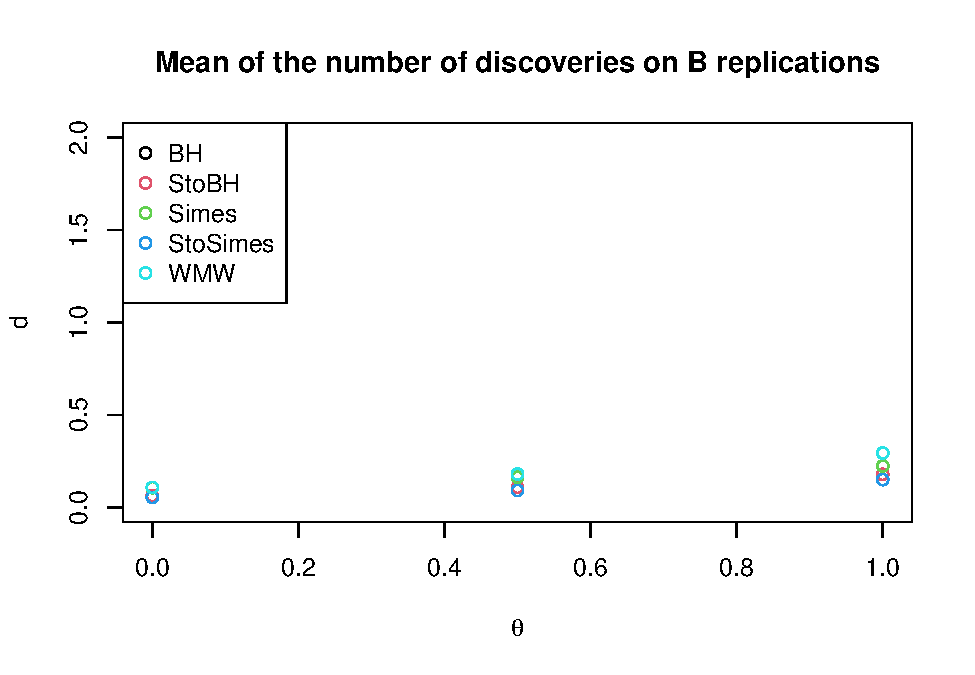
\includegraphics{LMPIresults_files/figure-latex/unnamed-chunk-2-1.pdf}

\begin{Shaded}
\begin{Highlighting}[]
\FunctionTok{plot}\NormalTok{(}\AttributeTok{x =}\NormalTok{ thetas, }\AttributeTok{y =}\NormalTok{ store\_res}\SpecialCharTok{$}\NormalTok{mean.powerGlobalNull[,}\DecValTok{1}\NormalTok{], }\AttributeTok{col =} \DecValTok{1}\NormalTok{, }\AttributeTok{ylab =} \StringTok{"power"}\NormalTok{, }
     \AttributeTok{xlab =} \FunctionTok{expression}\NormalTok{(theta), }\AttributeTok{ylim=}\FunctionTok{c}\NormalTok{(}\DecValTok{0}\NormalTok{,m),}
     \AttributeTok{main =} \StringTok{"Mean of the power on B replications"}\NormalTok{)}
\FunctionTok{points}\NormalTok{(}\AttributeTok{x =}\NormalTok{ thetas, }\AttributeTok{y =}\NormalTok{ store\_res}\SpecialCharTok{$}\NormalTok{mean.powerGlobalNull[,}\DecValTok{2}\NormalTok{], }\AttributeTok{col =} \DecValTok{2}\NormalTok{)}
\FunctionTok{points}\NormalTok{(}\AttributeTok{x =}\NormalTok{ thetas, }\AttributeTok{y =}\NormalTok{ store\_res}\SpecialCharTok{$}\NormalTok{mean.powerGlobalNull[,}\DecValTok{3}\NormalTok{], }\AttributeTok{col =} \DecValTok{3}\NormalTok{)}
\FunctionTok{points}\NormalTok{(}\AttributeTok{x =}\NormalTok{ thetas, }\AttributeTok{y =}\NormalTok{ store\_res}\SpecialCharTok{$}\NormalTok{mean.powerGlobalNull[,}\DecValTok{4}\NormalTok{], }\AttributeTok{col =} \DecValTok{4}\NormalTok{)}
\FunctionTok{points}\NormalTok{(}\AttributeTok{x =}\NormalTok{ thetas, }\AttributeTok{y =}\NormalTok{ store\_res}\SpecialCharTok{$}\NormalTok{mean.powerGlobalNull[,}\DecValTok{5}\NormalTok{], }\AttributeTok{col =} \DecValTok{5}\NormalTok{)}
\FunctionTok{legend}\NormalTok{(}\StringTok{"topleft"}\NormalTok{, }\AttributeTok{pch =} \DecValTok{1}\NormalTok{, }\AttributeTok{legend =} \FunctionTok{colnames}\NormalTok{(store\_res}\SpecialCharTok{$}\NormalTok{mean.powerGlobalNull), }\AttributeTok{col =} \FunctionTok{c}\NormalTok{(}\DecValTok{1}\NormalTok{,}\DecValTok{2}\NormalTok{,}\DecValTok{3}\NormalTok{,}\DecValTok{4}\NormalTok{,}\DecValTok{5}\NormalTok{))}
\end{Highlighting}
\end{Shaded}

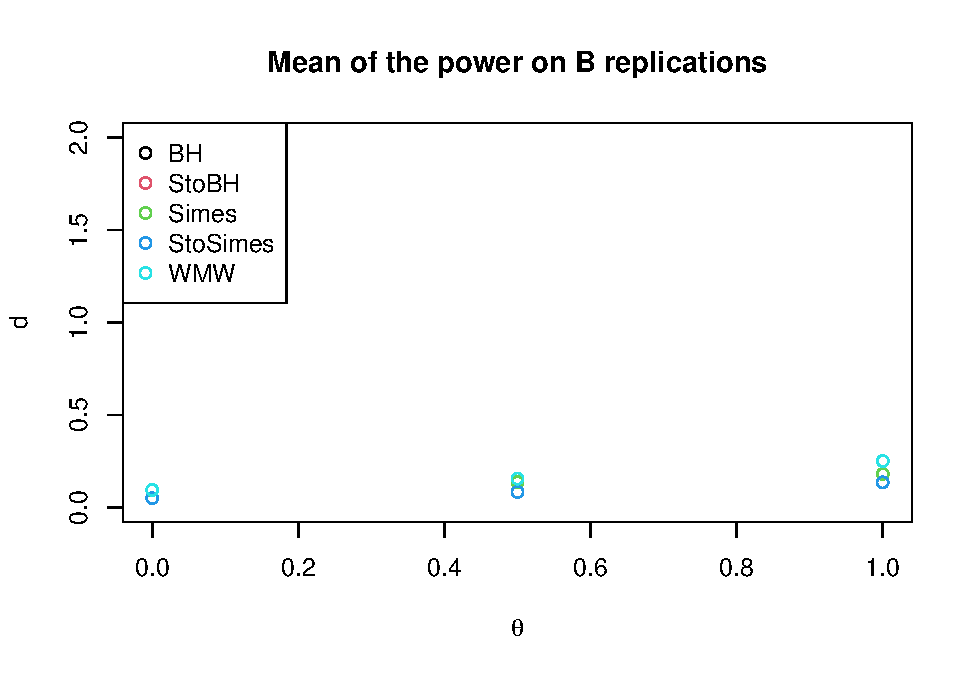
\includegraphics{LMPIresults_files/figure-latex/unnamed-chunk-2-2.pdf}

\hypertarget{k3}{%
\subsubsection{K=3}\label{k3}}

\begin{Shaded}
\begin{Highlighting}[]
\FunctionTok{set.seed}\NormalTok{(}\DecValTok{321}\NormalTok{)}

\CommentTok{\# Initializing parameters}
\NormalTok{B}\OtherTok{=}\DecValTok{10}\SpecialCharTok{\^{}}\DecValTok{5}
\NormalTok{n }\OtherTok{=} \DecValTok{19}
\NormalTok{l }\OtherTok{=} \DecValTok{19}
\NormalTok{m }\OtherTok{=} \DecValTok{2}
\NormalTok{d }\OtherTok{=} \DecValTok{3}
\NormalTok{k }\OtherTok{=} \DecValTok{3}
\NormalTok{alpha }\OtherTok{=}\NormalTok{ m}\SpecialCharTok{/}\NormalTok{(n}\SpecialCharTok{+}\DecValTok{1}\NormalTok{)}
\NormalTok{m1s }\OtherTok{=} \FunctionTok{seq}\NormalTok{(}\AttributeTok{from=}\DecValTok{0}\NormalTok{, }\AttributeTok{to=}\NormalTok{m, }\AttributeTok{by=}\DecValTok{1}\NormalTok{)}
\NormalTok{thetas }\OtherTok{=}\NormalTok{ m1s}\SpecialCharTok{/}\NormalTok{m}

\CommentTok{\# Results}
\NormalTok{res }\OtherTok{=} \FunctionTok{lapply}\NormalTok{(thetas, }\ControlFlowTok{function}\NormalTok{(theta) }\FunctionTok{simuLMPI}\NormalTok{(}\AttributeTok{B=}\NormalTok{B, }\AttributeTok{n=}\NormalTok{n, }\AttributeTok{l=}\NormalTok{l, }\AttributeTok{m=}\NormalTok{m, }\AttributeTok{d =}\NormalTok{ d, }
                                              \AttributeTok{k =}\NormalTok{ k, theta, }\AttributeTok{alpha =}\NormalTok{ m}\SpecialCharTok{/}\NormalTok{(l}\SpecialCharTok{+}\DecValTok{1}\NormalTok{)))}

\CommentTok{\# Storing results}
\NormalTok{store\_res }\OtherTok{=} \FunctionTok{list}\NormalTok{(}\StringTok{"mean.discov"} \OtherTok{=} \FunctionTok{matrix}\NormalTok{(}\AttributeTok{nrow=}\FunctionTok{length}\NormalTok{(thetas), }\AttributeTok{ncol =} \DecValTok{5}\NormalTok{), }
                 \StringTok{"mean.powerGlobalNull"} \OtherTok{=} \FunctionTok{matrix}\NormalTok{(}\AttributeTok{nrow=}\FunctionTok{length}\NormalTok{(thetas), }\AttributeTok{ncol =} \DecValTok{5}\NormalTok{))}
\NormalTok{row.names }\OtherTok{=} \FunctionTok{rep}\NormalTok{(}\ConstantTok{NA}\NormalTok{, }\AttributeTok{times=}\FunctionTok{length}\NormalTok{(thetas))}
\ControlFlowTok{for}\NormalTok{(i }\ControlFlowTok{in} \DecValTok{1}\SpecialCharTok{:}\FunctionTok{length}\NormalTok{(thetas))\{}
\NormalTok{  row.names[i] }\OtherTok{=} \FunctionTok{paste}\NormalTok{(}\StringTok{"theta ="}\NormalTok{,thetas[i])}
\NormalTok{\}}
\FunctionTok{rownames}\NormalTok{(store\_res}\SpecialCharTok{$}\NormalTok{mean.discov) }\OtherTok{=}\NormalTok{ row.names  }
\FunctionTok{colnames}\NormalTok{(store\_res}\SpecialCharTok{$}\NormalTok{mean.discov) }\OtherTok{=} \FunctionTok{c}\NormalTok{(}\StringTok{"BH"}\NormalTok{, }\StringTok{"StoBH"}\NormalTok{, }\StringTok{"Simes"}\NormalTok{, }\StringTok{"StoSimes"}\NormalTok{, }\StringTok{"WMW"}\NormalTok{)}
\FunctionTok{rownames}\NormalTok{(store\_res}\SpecialCharTok{$}\NormalTok{mean.powerGlobalNull) }\OtherTok{=}\NormalTok{ row.names  }
\FunctionTok{colnames}\NormalTok{(store\_res}\SpecialCharTok{$}\NormalTok{mean.powerGlobalNull) }\OtherTok{=} \FunctionTok{c}\NormalTok{(}\StringTok{"BH"}\NormalTok{, }\StringTok{"StoBH"}\NormalTok{, }\StringTok{"Simes"}\NormalTok{, }\StringTok{"StoSimes"}\NormalTok{, }\StringTok{"WMW"}\NormalTok{)}


\ControlFlowTok{for}\NormalTok{(i }\ControlFlowTok{in} \DecValTok{1}\SpecialCharTok{:}\FunctionTok{length}\NormalTok{(res))\{}
\NormalTok{  store\_res}\SpecialCharTok{$}\NormalTok{mean.discov[i,] }\OtherTok{=}\NormalTok{ res[[i]]}\SpecialCharTok{$}\NormalTok{mean.discov}
\NormalTok{  store\_res}\SpecialCharTok{$}\NormalTok{mean.powerGlobalNull[i,] }\OtherTok{=}\NormalTok{ res[[i]]}\SpecialCharTok{$}\NormalTok{mean.powerGlobalNull}
\NormalTok{\}}

\NormalTok{store\_res}\SpecialCharTok{$}\NormalTok{mean.discov}
\end{Highlighting}
\end{Shaded}

\begin{verbatim}
##                  BH   StoBH   Simes StoSimes     WMW
## theta = 0   0.10359 0.06030 0.10359  0.05102 0.10451
## theta = 0.5 0.21311 0.14517 0.21311  0.12188 0.23430
## theta = 1   0.33588 0.30422 0.33588  0.24832 0.49315
\end{verbatim}

\begin{Shaded}
\begin{Highlighting}[]
\NormalTok{store\_res}\SpecialCharTok{$}\NormalTok{mean.powerGlobalNull}
\end{Highlighting}
\end{Shaded}

\begin{verbatim}
##                  BH   StoBH   Simes StoSimes     WMW
## theta = 0   0.09038 0.04709 0.09038  0.04709 0.09130
## theta = 0.5 0.17789 0.10995 0.17789  0.10995 0.19908
## theta = 1   0.25003 0.21837 0.25003  0.21837 0.40730
\end{verbatim}

\begin{Shaded}
\begin{Highlighting}[]
\FunctionTok{plot}\NormalTok{(}\AttributeTok{x =}\NormalTok{ thetas, }\AttributeTok{y =}\NormalTok{ store\_res}\SpecialCharTok{$}\NormalTok{mean.discov[,}\DecValTok{1}\NormalTok{], }\AttributeTok{col =} \DecValTok{1}\NormalTok{, }\AttributeTok{ylab =} \StringTok{"d"}\NormalTok{, }
     \AttributeTok{xlab =} \FunctionTok{expression}\NormalTok{(theta), }\AttributeTok{ylim=}\FunctionTok{c}\NormalTok{(}\DecValTok{0}\NormalTok{,m),}
     \AttributeTok{main =} \StringTok{"Mean of the number of discoveries on B replications"}\NormalTok{)}
\FunctionTok{points}\NormalTok{(}\AttributeTok{x =}\NormalTok{ thetas, }\AttributeTok{y =}\NormalTok{ store\_res}\SpecialCharTok{$}\NormalTok{mean.discov[,}\DecValTok{2}\NormalTok{], }\AttributeTok{col =} \DecValTok{2}\NormalTok{)}
\FunctionTok{points}\NormalTok{(}\AttributeTok{x =}\NormalTok{ thetas, }\AttributeTok{y =}\NormalTok{ store\_res}\SpecialCharTok{$}\NormalTok{mean.discov[,}\DecValTok{3}\NormalTok{], }\AttributeTok{col =} \DecValTok{3}\NormalTok{)}
\FunctionTok{points}\NormalTok{(}\AttributeTok{x =}\NormalTok{ thetas, }\AttributeTok{y =}\NormalTok{ store\_res}\SpecialCharTok{$}\NormalTok{mean.discov[,}\DecValTok{4}\NormalTok{], }\AttributeTok{col =} \DecValTok{4}\NormalTok{)}
\FunctionTok{points}\NormalTok{(}\AttributeTok{x =}\NormalTok{ thetas, }\AttributeTok{y =}\NormalTok{ store\_res}\SpecialCharTok{$}\NormalTok{mean.discov[,}\DecValTok{5}\NormalTok{], }\AttributeTok{col =} \DecValTok{5}\NormalTok{)}
\FunctionTok{legend}\NormalTok{(}\StringTok{"topleft"}\NormalTok{, }\AttributeTok{pch =} \DecValTok{1}\NormalTok{, }\AttributeTok{legend =} \FunctionTok{colnames}\NormalTok{(store\_res}\SpecialCharTok{$}\NormalTok{mean.discov), }\AttributeTok{col =} \FunctionTok{c}\NormalTok{(}\DecValTok{1}\NormalTok{,}\DecValTok{2}\NormalTok{,}\DecValTok{3}\NormalTok{,}\DecValTok{4}\NormalTok{,}\DecValTok{5}\NormalTok{))}
\end{Highlighting}
\end{Shaded}

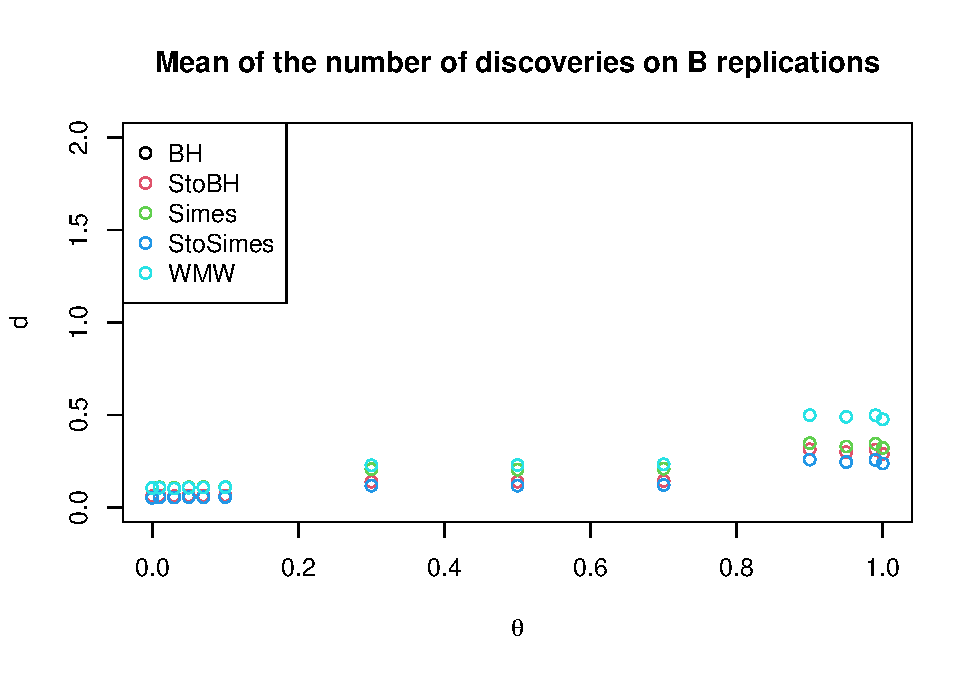
\includegraphics{LMPIresults_files/figure-latex/unnamed-chunk-3-1.pdf}

\begin{Shaded}
\begin{Highlighting}[]
\FunctionTok{plot}\NormalTok{(}\AttributeTok{x =}\NormalTok{ thetas, }\AttributeTok{y =}\NormalTok{ store\_res}\SpecialCharTok{$}\NormalTok{mean.powerGlobalNull[,}\DecValTok{1}\NormalTok{], }\AttributeTok{col =} \DecValTok{1}\NormalTok{, }\AttributeTok{ylab =} \StringTok{"power"}\NormalTok{, }
     \AttributeTok{xlab =} \FunctionTok{expression}\NormalTok{(theta), }\AttributeTok{ylim=}\FunctionTok{c}\NormalTok{(}\DecValTok{0}\NormalTok{,m),}
     \AttributeTok{main =} \StringTok{"Mean of the power on B replications"}\NormalTok{)}
\FunctionTok{points}\NormalTok{(}\AttributeTok{x =}\NormalTok{ thetas, }\AttributeTok{y =}\NormalTok{ store\_res}\SpecialCharTok{$}\NormalTok{mean.powerGlobalNull[,}\DecValTok{2}\NormalTok{], }\AttributeTok{col =} \DecValTok{2}\NormalTok{)}
\FunctionTok{points}\NormalTok{(}\AttributeTok{x =}\NormalTok{ thetas, }\AttributeTok{y =}\NormalTok{ store\_res}\SpecialCharTok{$}\NormalTok{mean.powerGlobalNull[,}\DecValTok{3}\NormalTok{], }\AttributeTok{col =} \DecValTok{3}\NormalTok{)}
\FunctionTok{points}\NormalTok{(}\AttributeTok{x =}\NormalTok{ thetas, }\AttributeTok{y =}\NormalTok{ store\_res}\SpecialCharTok{$}\NormalTok{mean.powerGlobalNull[,}\DecValTok{4}\NormalTok{], }\AttributeTok{col =} \DecValTok{4}\NormalTok{)}
\FunctionTok{points}\NormalTok{(}\AttributeTok{x =}\NormalTok{ thetas, }\AttributeTok{y =}\NormalTok{ store\_res}\SpecialCharTok{$}\NormalTok{mean.powerGlobalNull[,}\DecValTok{5}\NormalTok{], }\AttributeTok{col =} \DecValTok{5}\NormalTok{)}
\FunctionTok{legend}\NormalTok{(}\StringTok{"topleft"}\NormalTok{, }\AttributeTok{pch =} \DecValTok{1}\NormalTok{, }\AttributeTok{legend =} \FunctionTok{colnames}\NormalTok{(store\_res}\SpecialCharTok{$}\NormalTok{mean.powerGlobalNull), }\AttributeTok{col =} \FunctionTok{c}\NormalTok{(}\DecValTok{1}\NormalTok{,}\DecValTok{2}\NormalTok{,}\DecValTok{3}\NormalTok{,}\DecValTok{4}\NormalTok{,}\DecValTok{5}\NormalTok{))}
\end{Highlighting}
\end{Shaded}

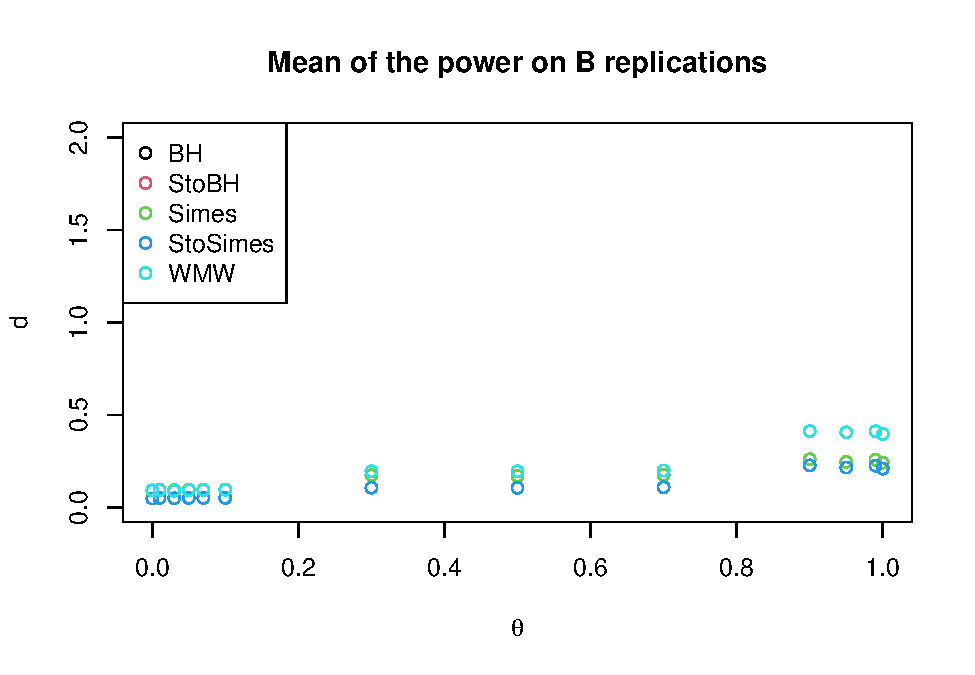
\includegraphics{LMPIresults_files/figure-latex/unnamed-chunk-3-2.pdf}

\hypertarget{k5}{%
\subsubsection{K=5}\label{k5}}

\begin{Shaded}
\begin{Highlighting}[]
\FunctionTok{set.seed}\NormalTok{(}\DecValTok{321}\NormalTok{)}

\CommentTok{\# Initializing parameters}
\NormalTok{B}\OtherTok{=}\DecValTok{10}\SpecialCharTok{\^{}}\DecValTok{5}
\NormalTok{n }\OtherTok{=} \DecValTok{19}
\NormalTok{l }\OtherTok{=} \DecValTok{19}
\NormalTok{m }\OtherTok{=} \DecValTok{2}
\NormalTok{d }\OtherTok{=} \DecValTok{3}
\NormalTok{k }\OtherTok{=} \DecValTok{5}
\NormalTok{alpha }\OtherTok{=}\NormalTok{ m}\SpecialCharTok{/}\NormalTok{(l}\SpecialCharTok{+}\DecValTok{1}\NormalTok{)}
\NormalTok{m1s }\OtherTok{=} \FunctionTok{seq}\NormalTok{(}\AttributeTok{from=}\DecValTok{0}\NormalTok{, }\AttributeTok{to=}\NormalTok{m, }\AttributeTok{by=}\DecValTok{1}\NormalTok{)}
\NormalTok{thetas }\OtherTok{=}\NormalTok{ m1s}\SpecialCharTok{/}\NormalTok{m}
\CommentTok{\# Results}
\NormalTok{res }\OtherTok{=} \FunctionTok{lapply}\NormalTok{(thetas, }\ControlFlowTok{function}\NormalTok{(theta) }\FunctionTok{simuLMPI}\NormalTok{(}\AttributeTok{B=}\NormalTok{B, }\AttributeTok{n=}\NormalTok{n, }\AttributeTok{l=}\NormalTok{l, }\AttributeTok{m=}\NormalTok{m, }\AttributeTok{d =}\NormalTok{ d, }
                                              \AttributeTok{k =}\NormalTok{ k, theta, }\AttributeTok{alpha =}\NormalTok{ m}\SpecialCharTok{/}\NormalTok{(l}\SpecialCharTok{+}\DecValTok{1}\NormalTok{)))}

\CommentTok{\# Storing results}
\NormalTok{store\_res }\OtherTok{=} \FunctionTok{list}\NormalTok{(}\StringTok{"mean.discov"} \OtherTok{=} \FunctionTok{matrix}\NormalTok{(}\AttributeTok{nrow=}\FunctionTok{length}\NormalTok{(thetas), }\AttributeTok{ncol =} \DecValTok{5}\NormalTok{), }
                 \StringTok{"mean.powerGlobalNull"} \OtherTok{=} \FunctionTok{matrix}\NormalTok{(}\AttributeTok{nrow=}\FunctionTok{length}\NormalTok{(thetas), }\AttributeTok{ncol =} \DecValTok{5}\NormalTok{))}
\NormalTok{row.names }\OtherTok{=} \FunctionTok{rep}\NormalTok{(}\ConstantTok{NA}\NormalTok{, }\AttributeTok{times=}\FunctionTok{length}\NormalTok{(thetas))}
\ControlFlowTok{for}\NormalTok{(i }\ControlFlowTok{in} \DecValTok{1}\SpecialCharTok{:}\FunctionTok{length}\NormalTok{(thetas))\{}
\NormalTok{  row.names[i] }\OtherTok{=} \FunctionTok{paste}\NormalTok{(}\StringTok{"theta ="}\NormalTok{,thetas[i])}
\NormalTok{\}}
\FunctionTok{rownames}\NormalTok{(store\_res}\SpecialCharTok{$}\NormalTok{mean.discov) }\OtherTok{=}\NormalTok{ row.names  }
\FunctionTok{colnames}\NormalTok{(store\_res}\SpecialCharTok{$}\NormalTok{mean.discov) }\OtherTok{=} \FunctionTok{c}\NormalTok{(}\StringTok{"BH"}\NormalTok{, }\StringTok{"StoBH"}\NormalTok{, }\StringTok{"Simes"}\NormalTok{, }\StringTok{"StoSimes"}\NormalTok{, }\StringTok{"WMW"}\NormalTok{)}
\FunctionTok{rownames}\NormalTok{(store\_res}\SpecialCharTok{$}\NormalTok{mean.powerGlobalNull) }\OtherTok{=}\NormalTok{ row.names  }
\FunctionTok{colnames}\NormalTok{(store\_res}\SpecialCharTok{$}\NormalTok{mean.powerGlobalNull) }\OtherTok{=} \FunctionTok{c}\NormalTok{(}\StringTok{"BH"}\NormalTok{, }\StringTok{"StoBH"}\NormalTok{, }\StringTok{"Simes"}\NormalTok{, }\StringTok{"StoSimes"}\NormalTok{, }\StringTok{"WMW"}\NormalTok{)}


\ControlFlowTok{for}\NormalTok{(i }\ControlFlowTok{in} \DecValTok{1}\SpecialCharTok{:}\FunctionTok{length}\NormalTok{(res))\{}
\NormalTok{  store\_res}\SpecialCharTok{$}\NormalTok{mean.discov[i,] }\OtherTok{=}\NormalTok{ res[[i]]}\SpecialCharTok{$}\NormalTok{mean.discov}
\NormalTok{  store\_res}\SpecialCharTok{$}\NormalTok{mean.powerGlobalNull[i,] }\OtherTok{=}\NormalTok{ res[[i]]}\SpecialCharTok{$}\NormalTok{mean.powerGlobalNull}
\NormalTok{\}}

\NormalTok{store\_res}\SpecialCharTok{$}\NormalTok{mean.discov}
\end{Highlighting}
\end{Shaded}

\begin{verbatim}
##                  BH   StoBH   Simes StoSimes     WMW
## theta = 0   0.10679 0.06158 0.10679  0.05258 0.10495
## theta = 0.5 0.28975 0.19300 0.28975  0.16252 0.29814
## theta = 1   0.54767 0.53166 0.54767  0.42445 0.81167
\end{verbatim}

\begin{Shaded}
\begin{Highlighting}[]
\NormalTok{store\_res}\SpecialCharTok{$}\NormalTok{mean.powerGlobalNull}
\end{Highlighting}
\end{Shaded}

\begin{verbatim}
##                  BH   StoBH   Simes StoSimes     WMW
## theta = 0   0.09370 0.04849 0.09370  0.04849 0.09186
## theta = 0.5 0.24255 0.14580 0.24255  0.14580 0.25094
## theta = 1   0.37586 0.35985 0.37586  0.35985 0.63986
\end{verbatim}

\begin{Shaded}
\begin{Highlighting}[]
\FunctionTok{plot}\NormalTok{(}\AttributeTok{x =}\NormalTok{ thetas, }\AttributeTok{y =}\NormalTok{ store\_res}\SpecialCharTok{$}\NormalTok{mean.discov[,}\DecValTok{1}\NormalTok{], }\AttributeTok{col =} \DecValTok{1}\NormalTok{, }\AttributeTok{ylab =} \StringTok{"d"}\NormalTok{, }
     \AttributeTok{xlab =} \FunctionTok{expression}\NormalTok{(theta), }\AttributeTok{ylim=}\FunctionTok{c}\NormalTok{(}\DecValTok{0}\NormalTok{,m),}
     \AttributeTok{main =} \StringTok{"Mean of the number of discoveries on B replications"}\NormalTok{)}
\FunctionTok{points}\NormalTok{(}\AttributeTok{x =}\NormalTok{ thetas, }\AttributeTok{y =}\NormalTok{ store\_res}\SpecialCharTok{$}\NormalTok{mean.discov[,}\DecValTok{2}\NormalTok{], }\AttributeTok{col =} \DecValTok{2}\NormalTok{)}
\FunctionTok{points}\NormalTok{(}\AttributeTok{x =}\NormalTok{ thetas, }\AttributeTok{y =}\NormalTok{ store\_res}\SpecialCharTok{$}\NormalTok{mean.discov[,}\DecValTok{3}\NormalTok{], }\AttributeTok{col =} \DecValTok{3}\NormalTok{)}
\FunctionTok{points}\NormalTok{(}\AttributeTok{x =}\NormalTok{ thetas, }\AttributeTok{y =}\NormalTok{ store\_res}\SpecialCharTok{$}\NormalTok{mean.discov[,}\DecValTok{4}\NormalTok{], }\AttributeTok{col =} \DecValTok{4}\NormalTok{)}
\FunctionTok{points}\NormalTok{(}\AttributeTok{x =}\NormalTok{ thetas, }\AttributeTok{y =}\NormalTok{ store\_res}\SpecialCharTok{$}\NormalTok{mean.discov[,}\DecValTok{5}\NormalTok{], }\AttributeTok{col =} \DecValTok{5}\NormalTok{)}
\FunctionTok{legend}\NormalTok{(}\StringTok{"topleft"}\NormalTok{, }\AttributeTok{pch =} \DecValTok{1}\NormalTok{, }\AttributeTok{legend =} \FunctionTok{colnames}\NormalTok{(store\_res}\SpecialCharTok{$}\NormalTok{mean.discov), }\AttributeTok{col =} \FunctionTok{c}\NormalTok{(}\DecValTok{1}\NormalTok{,}\DecValTok{2}\NormalTok{,}\DecValTok{3}\NormalTok{,}\DecValTok{4}\NormalTok{,}\DecValTok{5}\NormalTok{))}
\end{Highlighting}
\end{Shaded}

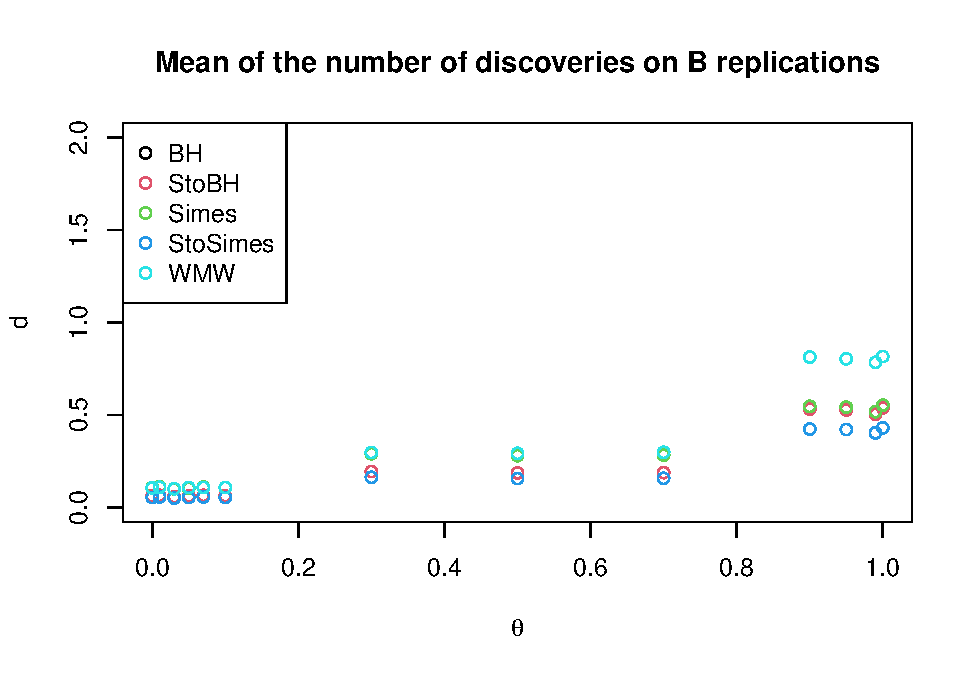
\includegraphics{LMPIresults_files/figure-latex/unnamed-chunk-4-1.pdf}

\begin{Shaded}
\begin{Highlighting}[]
\FunctionTok{plot}\NormalTok{(}\AttributeTok{x =}\NormalTok{ thetas, }\AttributeTok{y =}\NormalTok{ store\_res}\SpecialCharTok{$}\NormalTok{mean.powerGlobalNull[,}\DecValTok{1}\NormalTok{], }\AttributeTok{col =} \DecValTok{1}\NormalTok{, }\AttributeTok{ylab =} \StringTok{"power"}\NormalTok{, }
     \AttributeTok{xlab =} \FunctionTok{expression}\NormalTok{(theta), }\AttributeTok{ylim=}\FunctionTok{c}\NormalTok{(}\DecValTok{0}\NormalTok{,m),}
     \AttributeTok{main =} \StringTok{"Mean of the power on B replications"}\NormalTok{)}
\FunctionTok{points}\NormalTok{(}\AttributeTok{x =}\NormalTok{ thetas, }\AttributeTok{y =}\NormalTok{ store\_res}\SpecialCharTok{$}\NormalTok{mean.powerGlobalNull[,}\DecValTok{2}\NormalTok{], }\AttributeTok{col =} \DecValTok{2}\NormalTok{)}
\FunctionTok{points}\NormalTok{(}\AttributeTok{x =}\NormalTok{ thetas, }\AttributeTok{y =}\NormalTok{ store\_res}\SpecialCharTok{$}\NormalTok{mean.powerGlobalNull[,}\DecValTok{3}\NormalTok{], }\AttributeTok{col =} \DecValTok{3}\NormalTok{)}
\FunctionTok{points}\NormalTok{(}\AttributeTok{x =}\NormalTok{ thetas, }\AttributeTok{y =}\NormalTok{ store\_res}\SpecialCharTok{$}\NormalTok{mean.powerGlobalNull[,}\DecValTok{4}\NormalTok{], }\AttributeTok{col =} \DecValTok{4}\NormalTok{)}
\FunctionTok{points}\NormalTok{(}\AttributeTok{x =}\NormalTok{ thetas, }\AttributeTok{y =}\NormalTok{ store\_res}\SpecialCharTok{$}\NormalTok{mean.powerGlobalNull[,}\DecValTok{5}\NormalTok{], }\AttributeTok{col =} \DecValTok{5}\NormalTok{)}
\FunctionTok{legend}\NormalTok{(}\StringTok{"topleft"}\NormalTok{, }\AttributeTok{pch =} \DecValTok{1}\NormalTok{, }\AttributeTok{legend =} \FunctionTok{colnames}\NormalTok{(store\_res}\SpecialCharTok{$}\NormalTok{mean.powerGlobalNull), }\AttributeTok{col =} \FunctionTok{c}\NormalTok{(}\DecValTok{1}\NormalTok{,}\DecValTok{2}\NormalTok{,}\DecValTok{3}\NormalTok{,}\DecValTok{4}\NormalTok{,}\DecValTok{5}\NormalTok{))}
\end{Highlighting}
\end{Shaded}

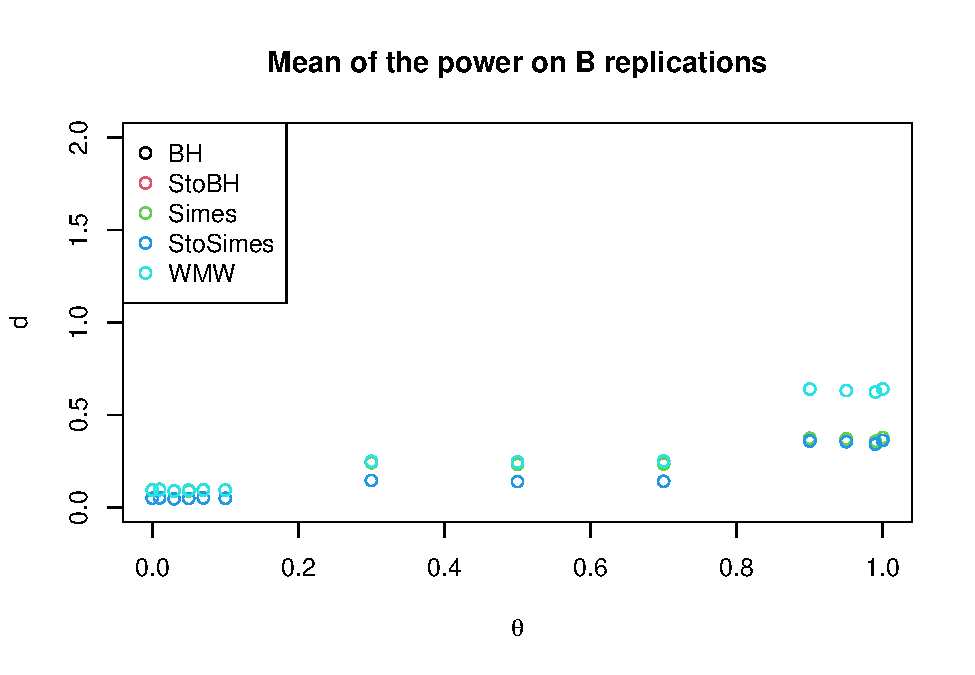
\includegraphics{LMPIresults_files/figure-latex/unnamed-chunk-4-2.pdf}

\hypertarget{k10}{%
\subsubsection{K=10}\label{k10}}

\begin{Shaded}
\begin{Highlighting}[]
\FunctionTok{set.seed}\NormalTok{(}\DecValTok{321}\NormalTok{)}

\CommentTok{\# Initializing parameters}
\NormalTok{B}\OtherTok{=}\DecValTok{10}\SpecialCharTok{\^{}}\DecValTok{5}
\NormalTok{n }\OtherTok{=} \DecValTok{19}
\NormalTok{l }\OtherTok{=} \DecValTok{19}
\NormalTok{m }\OtherTok{=} \DecValTok{2}
\NormalTok{d }\OtherTok{=} \DecValTok{3}
\NormalTok{k }\OtherTok{=} \DecValTok{10}
\NormalTok{alpha }\OtherTok{=}\NormalTok{ m}\SpecialCharTok{/}\NormalTok{(l}\SpecialCharTok{+}\DecValTok{1}\NormalTok{)}
\NormalTok{m1s }\OtherTok{=} \FunctionTok{seq}\NormalTok{(}\AttributeTok{from=}\DecValTok{0}\NormalTok{, }\AttributeTok{to=}\NormalTok{m, }\AttributeTok{by=}\DecValTok{1}\NormalTok{)}
\NormalTok{thetas }\OtherTok{=}\NormalTok{ m1s}\SpecialCharTok{/}\NormalTok{m}
\CommentTok{\# Results}
\NormalTok{res }\OtherTok{=} \FunctionTok{lapply}\NormalTok{(thetas, }\ControlFlowTok{function}\NormalTok{(theta) }\FunctionTok{simuLMPI}\NormalTok{(}\AttributeTok{B=}\NormalTok{B, }\AttributeTok{n=}\NormalTok{n, }\AttributeTok{l=}\NormalTok{l, }\AttributeTok{m=}\NormalTok{m, }\AttributeTok{d =}\NormalTok{ d, }
                                              \AttributeTok{k =}\NormalTok{ k, theta, }\AttributeTok{alpha =}\NormalTok{ m}\SpecialCharTok{/}\NormalTok{(l}\SpecialCharTok{+}\DecValTok{1}\NormalTok{)))}

\CommentTok{\# Storing results}
\NormalTok{store\_res }\OtherTok{=} \FunctionTok{list}\NormalTok{(}\StringTok{"mean.discov"} \OtherTok{=} \FunctionTok{matrix}\NormalTok{(}\AttributeTok{nrow=}\FunctionTok{length}\NormalTok{(thetas), }\AttributeTok{ncol =} \DecValTok{5}\NormalTok{), }
                 \StringTok{"mean.powerGlobalNull"} \OtherTok{=} \FunctionTok{matrix}\NormalTok{(}\AttributeTok{nrow=}\FunctionTok{length}\NormalTok{(thetas), }\AttributeTok{ncol =} \DecValTok{5}\NormalTok{))}
\NormalTok{row.names }\OtherTok{=} \FunctionTok{rep}\NormalTok{(}\ConstantTok{NA}\NormalTok{, }\AttributeTok{times=}\FunctionTok{length}\NormalTok{(thetas))}
\ControlFlowTok{for}\NormalTok{(i }\ControlFlowTok{in} \DecValTok{1}\SpecialCharTok{:}\FunctionTok{length}\NormalTok{(thetas))\{}
\NormalTok{  row.names[i] }\OtherTok{=} \FunctionTok{paste}\NormalTok{(}\StringTok{"theta ="}\NormalTok{,thetas[i])}
\NormalTok{\}}
\FunctionTok{rownames}\NormalTok{(store\_res}\SpecialCharTok{$}\NormalTok{mean.discov) }\OtherTok{=}\NormalTok{ row.names  }
\FunctionTok{colnames}\NormalTok{(store\_res}\SpecialCharTok{$}\NormalTok{mean.discov) }\OtherTok{=} \FunctionTok{c}\NormalTok{(}\StringTok{"BH"}\NormalTok{, }\StringTok{"StoBH"}\NormalTok{, }\StringTok{"Simes"}\NormalTok{, }\StringTok{"StoSimes"}\NormalTok{, }\StringTok{"WMW"}\NormalTok{)}
\FunctionTok{rownames}\NormalTok{(store\_res}\SpecialCharTok{$}\NormalTok{mean.powerGlobalNull) }\OtherTok{=}\NormalTok{ row.names  }
\FunctionTok{colnames}\NormalTok{(store\_res}\SpecialCharTok{$}\NormalTok{mean.powerGlobalNull) }\OtherTok{=} \FunctionTok{c}\NormalTok{(}\StringTok{"BH"}\NormalTok{, }\StringTok{"StoBH"}\NormalTok{, }\StringTok{"Simes"}\NormalTok{, }\StringTok{"StoSimes"}\NormalTok{, }\StringTok{"WMW"}\NormalTok{)}


\ControlFlowTok{for}\NormalTok{(i }\ControlFlowTok{in} \DecValTok{1}\SpecialCharTok{:}\FunctionTok{length}\NormalTok{(res))\{}
\NormalTok{  store\_res}\SpecialCharTok{$}\NormalTok{mean.discov[i,] }\OtherTok{=}\NormalTok{ res[[i]]}\SpecialCharTok{$}\NormalTok{mean.discov}
\NormalTok{  store\_res}\SpecialCharTok{$}\NormalTok{mean.powerGlobalNull[i,] }\OtherTok{=}\NormalTok{ res[[i]]}\SpecialCharTok{$}\NormalTok{mean.powerGlobalNull}
\NormalTok{\}}

\NormalTok{store\_res}\SpecialCharTok{$}\NormalTok{mean.discov}
\end{Highlighting}
\end{Shaded}

\begin{verbatim}
##                  BH   StoBH   Simes StoSimes     WMW
## theta = 0   0.10450 0.06109 0.10450  0.05167 0.10479
## theta = 0.5 0.42185 0.26844 0.42185  0.22660 0.37136
## theta = 1   0.93889 0.93671 0.93889  0.73183 1.24884
\end{verbatim}

\begin{Shaded}
\begin{Highlighting}[]
\NormalTok{store\_res}\SpecialCharTok{$}\NormalTok{mean.powerGlobalNull}
\end{Highlighting}
\end{Shaded}

\begin{verbatim}
##                  BH   StoBH   Simes StoSimes     WMW
## theta = 0   0.09112 0.04771 0.09112  0.04771 0.09141
## theta = 0.5 0.35480 0.20139 0.35480  0.20139 0.30431
## theta = 1   0.57199 0.56981 0.57199  0.56981 0.88194
\end{verbatim}

\begin{Shaded}
\begin{Highlighting}[]
\FunctionTok{plot}\NormalTok{(}\AttributeTok{x =}\NormalTok{ thetas, }\AttributeTok{y =}\NormalTok{ store\_res}\SpecialCharTok{$}\NormalTok{mean.discov[,}\DecValTok{1}\NormalTok{], }\AttributeTok{col =} \DecValTok{1}\NormalTok{, }\AttributeTok{ylab =} \StringTok{"d"}\NormalTok{, }
     \AttributeTok{xlab =} \FunctionTok{expression}\NormalTok{(theta), }\AttributeTok{ylim=}\FunctionTok{c}\NormalTok{(}\DecValTok{0}\NormalTok{,m),}
     \AttributeTok{main =} \StringTok{"Mean of the number of discoveries on B replications"}\NormalTok{)}
\FunctionTok{points}\NormalTok{(}\AttributeTok{x =}\NormalTok{ thetas, }\AttributeTok{y =}\NormalTok{ store\_res}\SpecialCharTok{$}\NormalTok{mean.discov[,}\DecValTok{2}\NormalTok{], }\AttributeTok{col =} \DecValTok{2}\NormalTok{)}
\FunctionTok{points}\NormalTok{(}\AttributeTok{x =}\NormalTok{ thetas, }\AttributeTok{y =}\NormalTok{ store\_res}\SpecialCharTok{$}\NormalTok{mean.discov[,}\DecValTok{3}\NormalTok{], }\AttributeTok{col =} \DecValTok{3}\NormalTok{)}
\FunctionTok{points}\NormalTok{(}\AttributeTok{x =}\NormalTok{ thetas, }\AttributeTok{y =}\NormalTok{ store\_res}\SpecialCharTok{$}\NormalTok{mean.discov[,}\DecValTok{4}\NormalTok{], }\AttributeTok{col =} \DecValTok{4}\NormalTok{)}
\FunctionTok{points}\NormalTok{(}\AttributeTok{x =}\NormalTok{ thetas, }\AttributeTok{y =}\NormalTok{ store\_res}\SpecialCharTok{$}\NormalTok{mean.discov[,}\DecValTok{5}\NormalTok{], }\AttributeTok{col =} \DecValTok{5}\NormalTok{)}
\FunctionTok{legend}\NormalTok{(}\StringTok{"topleft"}\NormalTok{, }\AttributeTok{pch =} \DecValTok{1}\NormalTok{, }\AttributeTok{legend =} \FunctionTok{colnames}\NormalTok{(store\_res}\SpecialCharTok{$}\NormalTok{mean.discov), }\AttributeTok{col =} \FunctionTok{c}\NormalTok{(}\DecValTok{1}\NormalTok{,}\DecValTok{2}\NormalTok{,}\DecValTok{3}\NormalTok{,}\DecValTok{4}\NormalTok{,}\DecValTok{5}\NormalTok{))}
\end{Highlighting}
\end{Shaded}

\includegraphics{LMPIresults_files/figure-latex/unnamed-chunk-5-1.pdf}

\begin{Shaded}
\begin{Highlighting}[]
\FunctionTok{plot}\NormalTok{(}\AttributeTok{x =}\NormalTok{ thetas, }\AttributeTok{y =}\NormalTok{ store\_res}\SpecialCharTok{$}\NormalTok{mean.powerGlobalNull[,}\DecValTok{1}\NormalTok{], }\AttributeTok{col =} \DecValTok{1}\NormalTok{, }\AttributeTok{ylab =} \StringTok{"power"}\NormalTok{, }
     \AttributeTok{xlab =} \FunctionTok{expression}\NormalTok{(theta), }\AttributeTok{ylim=}\FunctionTok{c}\NormalTok{(}\DecValTok{0}\NormalTok{,m),}
     \AttributeTok{main =} \StringTok{"Mean of the power on B replications"}\NormalTok{)}
\FunctionTok{points}\NormalTok{(}\AttributeTok{x =}\NormalTok{ thetas, }\AttributeTok{y =}\NormalTok{ store\_res}\SpecialCharTok{$}\NormalTok{mean.powerGlobalNull[,}\DecValTok{2}\NormalTok{], }\AttributeTok{col =} \DecValTok{2}\NormalTok{)}
\FunctionTok{points}\NormalTok{(}\AttributeTok{x =}\NormalTok{ thetas, }\AttributeTok{y =}\NormalTok{ store\_res}\SpecialCharTok{$}\NormalTok{mean.powerGlobalNull[,}\DecValTok{3}\NormalTok{], }\AttributeTok{col =} \DecValTok{3}\NormalTok{)}
\FunctionTok{points}\NormalTok{(}\AttributeTok{x =}\NormalTok{ thetas, }\AttributeTok{y =}\NormalTok{ store\_res}\SpecialCharTok{$}\NormalTok{mean.powerGlobalNull[,}\DecValTok{4}\NormalTok{], }\AttributeTok{col =} \DecValTok{4}\NormalTok{)}
\FunctionTok{points}\NormalTok{(}\AttributeTok{x =}\NormalTok{ thetas, }\AttributeTok{y =}\NormalTok{ store\_res}\SpecialCharTok{$}\NormalTok{mean.powerGlobalNull[,}\DecValTok{5}\NormalTok{], }\AttributeTok{col =} \DecValTok{5}\NormalTok{)}
\FunctionTok{legend}\NormalTok{(}\StringTok{"topleft"}\NormalTok{, }\AttributeTok{pch =} \DecValTok{1}\NormalTok{, }\AttributeTok{legend =} \FunctionTok{colnames}\NormalTok{(store\_res}\SpecialCharTok{$}\NormalTok{mean.powerGlobalNull), }\AttributeTok{col =} \FunctionTok{c}\NormalTok{(}\DecValTok{1}\NormalTok{,}\DecValTok{2}\NormalTok{,}\DecValTok{3}\NormalTok{,}\DecValTok{4}\NormalTok{,}\DecValTok{5}\NormalTok{))}
\end{Highlighting}
\end{Shaded}

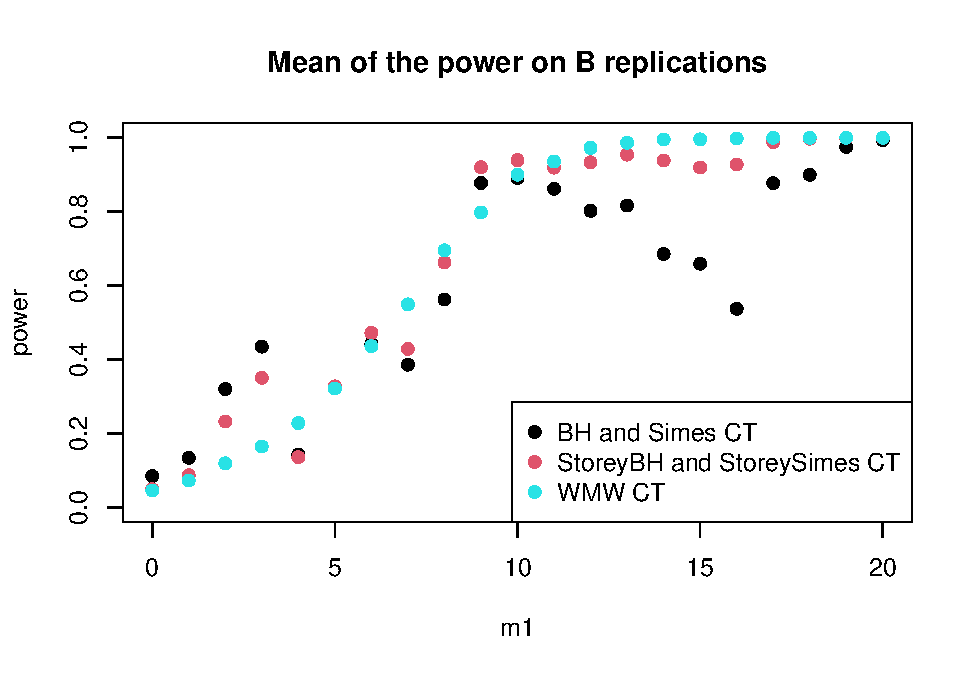
\includegraphics{LMPIresults_files/figure-latex/unnamed-chunk-5-2.pdf}

\end{document}
